\documentclass[11pt,a4paper]{article}
\usepackage[OT4]{polski}
\usepackage[utf8]{inputenc}
\usepackage[inner=2.5cm,outer=2.5cm, tmargin=2.5cm,bmargin=2.5cm]{geometry}
\usepackage{amsmath}
\usepackage{relsize,amsfonts}
\usepackage{enumitem}
\usepackage{graphicx}


  
\title{Bazy Danych\\\large \medskip Projekt\\}
\author{Mateusz Perciński Z59827}
\date{26 maja 2017}

\begin{document}

\maketitle
\tableofcontents

\section*{Treść projektu}
Zadanie zakłada zaprojektowanie i zaimplementowanie encji oraz relacji bazy danych aplikacji do nauki słówek, a także stworzenie podstawowych mechanizmów dynamicznych, które mogłyby znaleźć się w aplikacji tego typu. Dodatkowo, projekt zakłada napisanie prostej aplikacji w języku Java komunikującej się z bazą danych. 

\section{Projekt tabel}
Jaki był plan na bazę %TODO

Załącznik \ref{attach:delete-db} to skrypt SQL kasujący istniejące tabele oraz sekwencje, natomiast załącznik \ref{attach:create-db} - budujący bazę danych od początku. Tworzy tabele, definiuje klucze własne oraz obce, czyli zależności relacyjne miedzy encjami. Rysunek \ref{fig:model} przedstawia model relacyjny projektowanej bazy danych.

\begin{figure}[ht!]
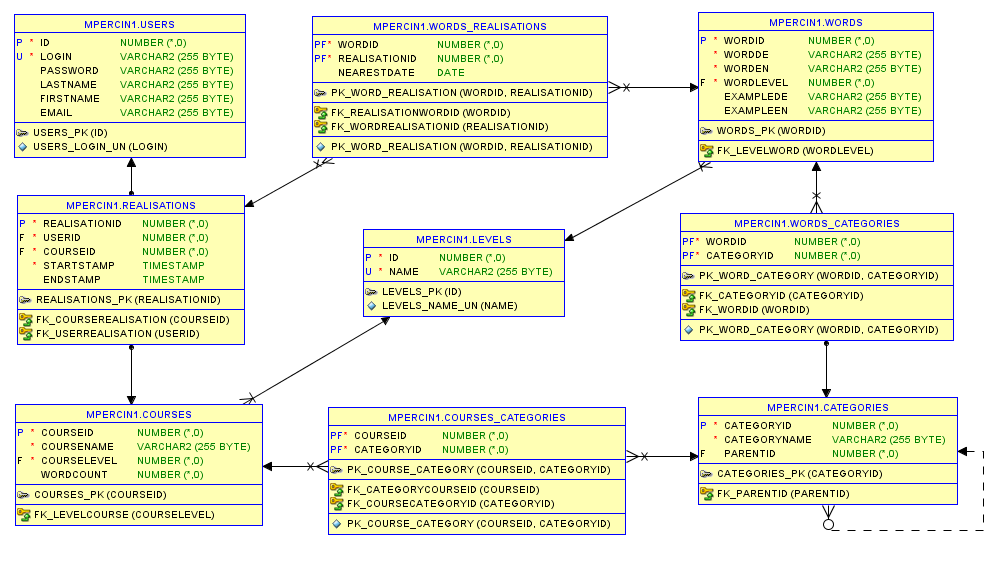
\includegraphics[width=\textwidth]{graphics/relational-model}
\caption{Model relacyjny bazy danych}
\label{fig:model}
\end{figure}

\section{Wstawianie danych}

\section{Generatory}

\section{Triggery}

\section{Zapytania SQL}

\section{Program w języku Java}

\section{Optymalizacja indeksów}

\section{Hinty}


\section*{Spis załączników}
\addcontentsline{toc}{section}{Spis załączników} 
\begin{enumerate}[label=\arabic*,ref=\arabic*]
\item \label{attach:create-db} \textit{delete-db.sql} - skrypt SQL usuwający wszystkie tabele oraz sekwencje
\item \label{attach:delete-db} \textit{create-db.sql} - skrypt SQL budujący hierarchię bazy danych
\end{enumerate}


\end{document}